%% project.tex
%% 2015/12/05
%% by Eric Scott Freeman
%% This document uses bare_jrnl_compsoc.tex template provided by Michael Shell.

\documentclass[10pt,journal,compsoc]{IEEEtran}

\ifCLASSOPTIONcompsoc
	% The IEEE Computer Society needs nocompress option
	% requires cite.sty v4.0 or later (November 2003)
	\usepackage[nocompress]{cite}
\else
	% normal IEEE
	\usepackage{cite}
\fi

\newcommand\MYhyperrefoptions{bookmarks=true,bookmarksnumbered=true,
	pdfpagemode={UseOutlines},plainpages=false,pdfpagelabels=true,
	colorlinks=true,linkcolor={black},citecolor={black},urlcolor={black},
	pdftitle={Anti-plagiarism Project},
	pdfsubject={Anti-plagiarism},
	pdfauthor={Eric Scott Freeman},
	pdfkeywords={anti-plagiarism, plagiarism, fingerprinting, stylometry, Moss, JPlag, dupl, Autograder}}

\usepackage{amssymb}                % For the checkmarks in the table
\usepackage{booktabs}               % For the table
\usepackage{floatrow}               % To make the images fit
\usepackage{graphicx}               % To show images
\usepackage{listings}
\usepackage{url}                    % For adding URLs
\usepackage[utf8]{inputenc}         % For displaying accented characters

% correct bad hyphenation here
\hyphenation{}

\begin{document}

	\title{Anti-plagiarism Project}
	\author{Eric~Scott~Freeman}

	\IEEEtitleabstractindextext{
	\begin{abstract}
	This project integrates several anti-plagiarism tools into Autograder, software used by the University of Stavanger to automatically grade students' programming assignments. The three tools used were good at finding duplicate pieces of code, but it is still up to the instructor to determine whether or not it could be considered plagiarism.
	\end{abstract}
		
	\begin{IEEEkeywords}
	anti-plagiarism, plagiarism, fingerprinting, stylometry, Moss, JPlag, dupl, Autograder.
	\end{IEEEkeywords}}

	\maketitle
	\IEEEdisplaynontitleabstractindextext
	\IEEEpeerreviewmaketitle

	\IEEEraisesectionheading{\section{Introduction}\label{sec:introduction}}
	
	\IEEEPARstart{A}{s} the number of students in Computer Science classes grow, instructors have less time to spend grading individual student programming assignments. So colleges and universities have started implementing software to help grade student assignments. The University of Stavanger uses an application called Autograder, written by Heine Furubotten, to automatically grade students' programming assignments.
	
	By using software to grade assignments, instructors may spend less time looking at them. Therefore it is more likely that plagiarism could escape detection. Several tools exist which can detect plagiarism in programming assignments.
	
	The goal of this project is to integrate a few anti-plagiarism tools into Autograder, since there currently is none. By integrating different tools, it will possible to compare them to see which one works the best. Additionally having multiple tools detect plagiarism in a student's assignment would provide more verification that the student had plagiarized the code.
	
	This paper will first discuss various methods for detecting plagiarism and existing tools in Section 2. Section 3 will explain the design of the project and how it is integrated with Autograder. Section 4 will present the results of running the anti-plagiarism project against real assignments submitted by students, and Section 5 will analyze the results. In Section 6, future work will be described.

	\section{Related Work}
	This section provides an overview of some of the techniques used in checking for plagiarism. It also describes Autograder. Unfortunately software plagiarism is a problem both in the classroom and in the workplace. A number of applications have been created to help detect this problem. While these tools can find similarities in programs, the flagged files must still be manually examined to determine whether or not code was plagiarized. There are several different general techniques that are used to look for plagiarism. The tools analyzed in this project used either fingerprinting or stylometry.
		
		\subsection{Fingerprinting}
		Several tools use a technique called fingerprinting to detect plagiarism. In fingerprinting algorithms, variable names are changed and extra whitespace is removed, which helps eliminate superficial changes to code. Then multiple hashes of $n$-grams, substrings that are $n$ characters, are saved and can compared to help find plagiarism. Matching hashes are then flagged as potential plagiarism. Not all hashes are stored due to the large number that would be produced.
		
			\subsubsection{Winnowing}
			Moss uses a technique called winnowing to select which hashes to save \cite{schleimer+wilkerson+aiken}. In the winnowing algorithm, a window, a selection of contiguous hashes, is used to help select which hashes to save. The smallest hash from a window is saved, and then the window moves one hash over. The smallest hash from the next window is often the smallest hash from the previous window. If so it is not saved again. This limits the number of hashes saved to the fingerprint, and the use of a window keeps the distance between hashes from becoming too large. A large distance increases the chance plagiarism being undetected. Figure \ref{fig:winnowing1} shows an example of how winnowing works. The orange box represents the shifting window. The green box shows whenever a new hash is saved.
		
			\begin{figure}[h!]
				\includegraphics[width=0.8\textwidth]{Winnowing.png}
				\caption{Winnowing.}
				\label{fig:winnowing1}
			\end{figure}
		
			\subsubsection{Running-Karp-Rabin Greedy-String-Tiling}
			JPlag uses Running-Karp-Rabin Greedy-String-Tiling (RKS-GST) to compare hashes of code in plagiarism detection \cite{prechelt+malpohl+philippsen}. RKS-GST was originally used in YAP3, another plagiarism detection tool. In RKS-GST, the Karp-Rabin half of the algorithm finds matching strings by comparing hashes in near linear time, and the Greedy-String-Tiling algorithm half makes sure that strings in the match are not part of another match \cite{wise}. It starts from the biggest match and goes down to the smallest. It was designed to help detect when students try to hide plagiarism by reordering code.
		
		\subsection{Stylometry}
		Another approach is to use code stylometry, which analyzes the style of writing or coding.
		
			\subsubsection{Abstract Syntax Trees}
			Caliskan-Islam, et al. use abstract syntax trees (ASTs) to compare the styles of authors \cite{caliskan-islam+harang+liu}. Things that are easily changed in code, such as variable names, become leaves in the AST, while the structure of the tree is harder to change \cite{caliskan-islam+harang+liu}. For example, if one student copied a function from another student and only changed the variable names, the structure of the tree would look exactly the same. This could then be flagged as potential plagiarism. Figure \ref{fig:ast} shows an abstract syntax tree of the code in Figure \ref{fig:astcode}. Note how the leaves, or circular nodes, in Figure \ref{fig:ast} are variable names, constants, and a function name.
		
			\begin{figure}
				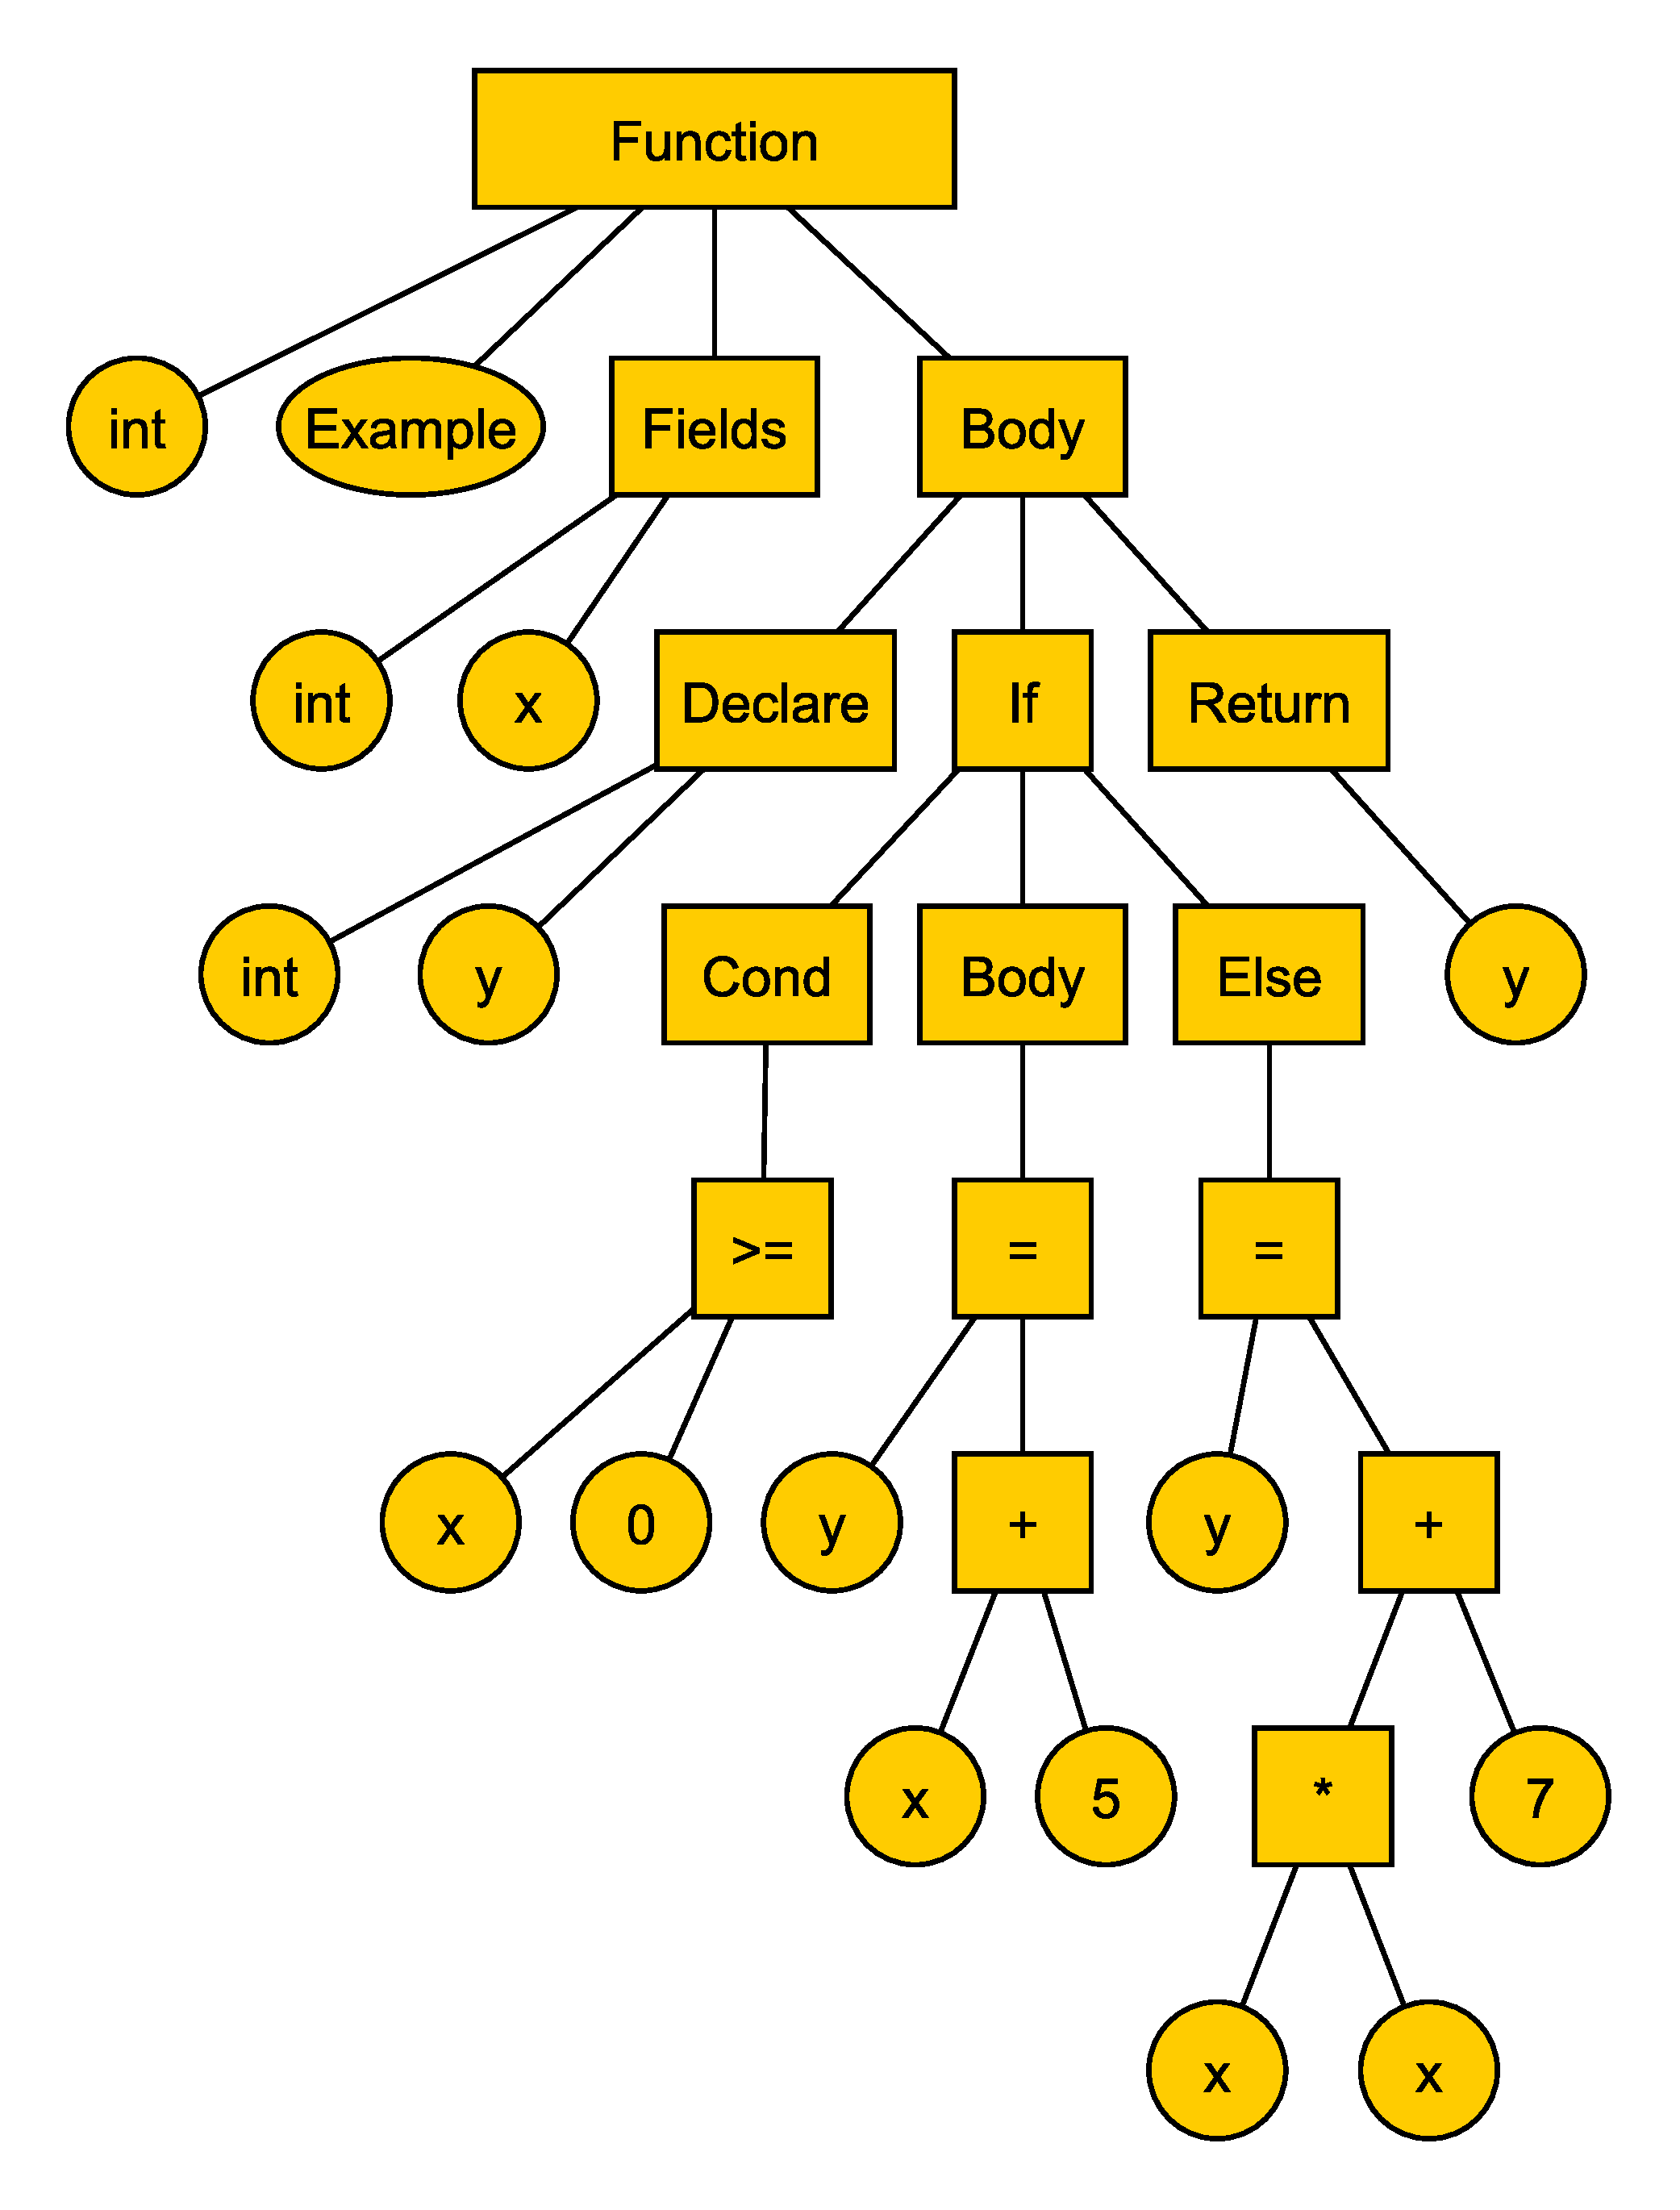
\includegraphics[width=0.8\textwidth]{AST.pdf}
				\caption{Abstract syntax tree.}
				\label{fig:ast}
			\end{figure}
			\begin{figure}
				\includegraphics[width=0.5\textwidth]{ASTcode.png}
				\caption{Example code.}
				\label{fig:astcode}
			\end{figure}
		
		\subsection{Autograder}
		Autograder was written for Heine Furubotten's Master's thesis, and it automatically grades students' programming assignments \cite{furubotten}. When a student is registered for a course with Autograder, GitHub will notify Autograder whenever the student pushes new code to the repository. Autograder will then create a Docker container to test the student's code. By using the Docker container, there is less chance of the student's code accidentally or purposely harming the Autograder server. Once the tests are complete, the results are stored in a Bolt database. Bolt stores entries as a key/value pair.
		
		Autograder also provides a web service which gives students feedback on their assignments. They are able to see how many of the tests had passed and why any tests had failed. Once a certain number of tests are passed, students can ask the instructors to approve the assignment. Instructors do this through the web interface provided to them. This also gives them an overview of how the whole class is doing on the assignments.
		
	\section{Design}
	This section describes some of the design decisions made during the development process and how a request to check the students' code for plagiarism works.
	
		\subsection{Selection of tools}
		Three tools were chosen for the project to use three different techniques for finding plagiarism: winnowing, RKS-GST, and ASTs. Table \ref{tab:languageSupport} shows the languages officially supported by several anti-plagiarism tools.
		
		\begin{table}[h!]
			\begin{center}
				\caption{Officially supported languages by various tools}
				\label{tab:languageSupport}
				\begin{tabular}{ccccccccccccccc}
					\toprule
					Tool & Java & Go & C & C\verb!++! & C\verb!#! & Python & others\\
					\midrule
					Moss & \checkmark & & \checkmark & \checkmark & \checkmark & \checkmark & \checkmark \\
					JPlag & \checkmark & & \checkmark & \checkmark & \checkmark & & \checkmark\\
					Plaggie & \checkmark & & & & & & \\
					dupl & & \checkmark & & & & & \\
					\bottomrule
				\end{tabular}
			\end{center}
		\end{table}
		
			\subsubsection{Moss}
			Moss is an anti-plagiarism tool which uses winnowing to find similar pieces of code. It was the first choice in anti-plagiarism tools, because it supports a large number of languages and is a mature piece of software. While Moss does not officially support Go, it can still check Go files. A very nice feature is its ability to ignore similar pieces of code if the it appears it a certain number of files. So code that is common to everyone, such as code provided by instructor, can be ignored. It is free to use the Moss service, but it requires registration. To run Moss locally, a fee must be paid.
		
			\subsubsection{JPlag}
			JPlag is an anti-plagiarism tool which uses RKS-GST to find similar code. Like Moss, JPlag supports many languages. It is free, open-source, and can be run locally. JPlag will only check files written in the languages it officially supports. While JPlag can ignore files, it must be told which files to ignore.
		
			\subsubsection{dupl}
			Michal Bohuslávek's dupl application uses ASTs to find similarities in code for big projects \cite{bohuslave}. Dupl was chosen for its use of ASTs, which means it uses stylometry instead of fingerprinting, and its support for the Go programming language. Dupl is free, open-source, and can be run locally. It will only work with Go files. Dupl looks for any copies of code, not just plagiarism. So if a piece of code is duplicated even in the same file, it will test positive. Since dupl was not designed to test for plagiarism, there is no way to tell it to ignore code. It also does not provide a percentage saying what percentage of code is likely to be plagiarized. The checked code must be able to compile since dupl needs to parse the code to make the ASTs correctly.
		
			\subsubsection{Tools not chosen}
			There are several tools which were not chosen. For example, Plaggie supports only Java, while the data from the test course was written in C and Go. So Plaggie would not have been a good choice.
		
		\subsection{Integrating with Autograder}
		Some changes needed to be made to Autograder before it would work with this project. A few new fields needed to be added to the Autograder's Bolt database. Each lab assignment entry in each class needed to store the language the assignment is written in. Also each lab assignment entry for each student/group needed to store the results from each of the anti-plagiarism tools.
		
		The user interface was also updated to allow teachers to assign a programming language to each lab (figure \ref{fig:selectLang}), to allow teachers to initiate the anti-plagiarism process (figure \ref{fig:startTest}), and to show the results of the process. 
		
		\begin{figure}[h!]
			\includegraphics[width=0.6\textwidth]{SelectingLanguage.png}
			\caption{Selecting language.}
			\label{fig:selectLang}
		\end{figure}
		
		\begin{figure}[h!]
			\includegraphics[width=0.6\textwidth]{StartTest.png}
			\caption{Start anti-plagiarism test.}
			\label{fig:startTest}
		\end{figure}
		
		The results are stored in the database and also displayed to the teachers through the teacher panel in Autograder. The teacher panel shows a table of all the students in the class and their assignments. If any of the anti-plagiarism tools find evidence of plagiarism, the corresponding cell in the table will be colored a shade of red. The more tools finding plagiarism, the deeper the color. From the teacher panel, teachers can go to a results page to look at more details about each lab. This page shows the results of each anti-plagiarism tool and buttons which link to the plagiarized code. See figure \ref{fig:labresults}.
		
		\begin{figure}[h!]
			\includegraphics[width=0.7\textwidth]{LabResults.png}
			\caption{Results for one lab.}
			\label{fig:labresults}
		\end{figure}
		
		While adding the new functionality to Autograder, care was taken not to break any existing functionality. Unit tests were rerun to check that nothing was broken.
		
		\subsection{Directory structure}
		The directory structure of the students' code consists of a base directory containing subdirectories for each class. Each class is a GitHub organization. Inside each class, there are directories for each student, which have directories for each assignment. See figure \ref{fig:directories}. This is similar to how Autograder stores the files in GitHub, so pulling the code for the anti-plagiarism project is simplified. This was a convenient way for organizing the code for processing by the different tools as well.
		
		\begin{figure}[h!]
			\includegraphics[width=0.4\textwidth]{Directories.png}
			\caption{Directory structure.}
			\label{fig:directories}
		\end{figure}

		\subsection{Process}
		Since Autograder was written in Go, this project was also written in Go. Later it was decided to make this project a standalone application that Autograder will call, since another university has expressed interest in using it. The program calls each of the anti-plagiarism tools and stores the results. A separate Go package was written for each anti-plagiarism tool. The packages implement a common interface which creates the commands to send to the tools and formats the results. The interface will allow other anti-plagiarism tools to be easily added later.
		
		The anti-plagiarism application typically runs as a service and accepts gRPC, a remote procedure call framework, requests. A request to check the students' code for plagiarism consists of the GitHub organization, the GitHub authorization token, an array of student repository names, and an array of lab assignment names and programming languages. Requests can also be sent from the command line.
		
		\begin{figure}[h!]
			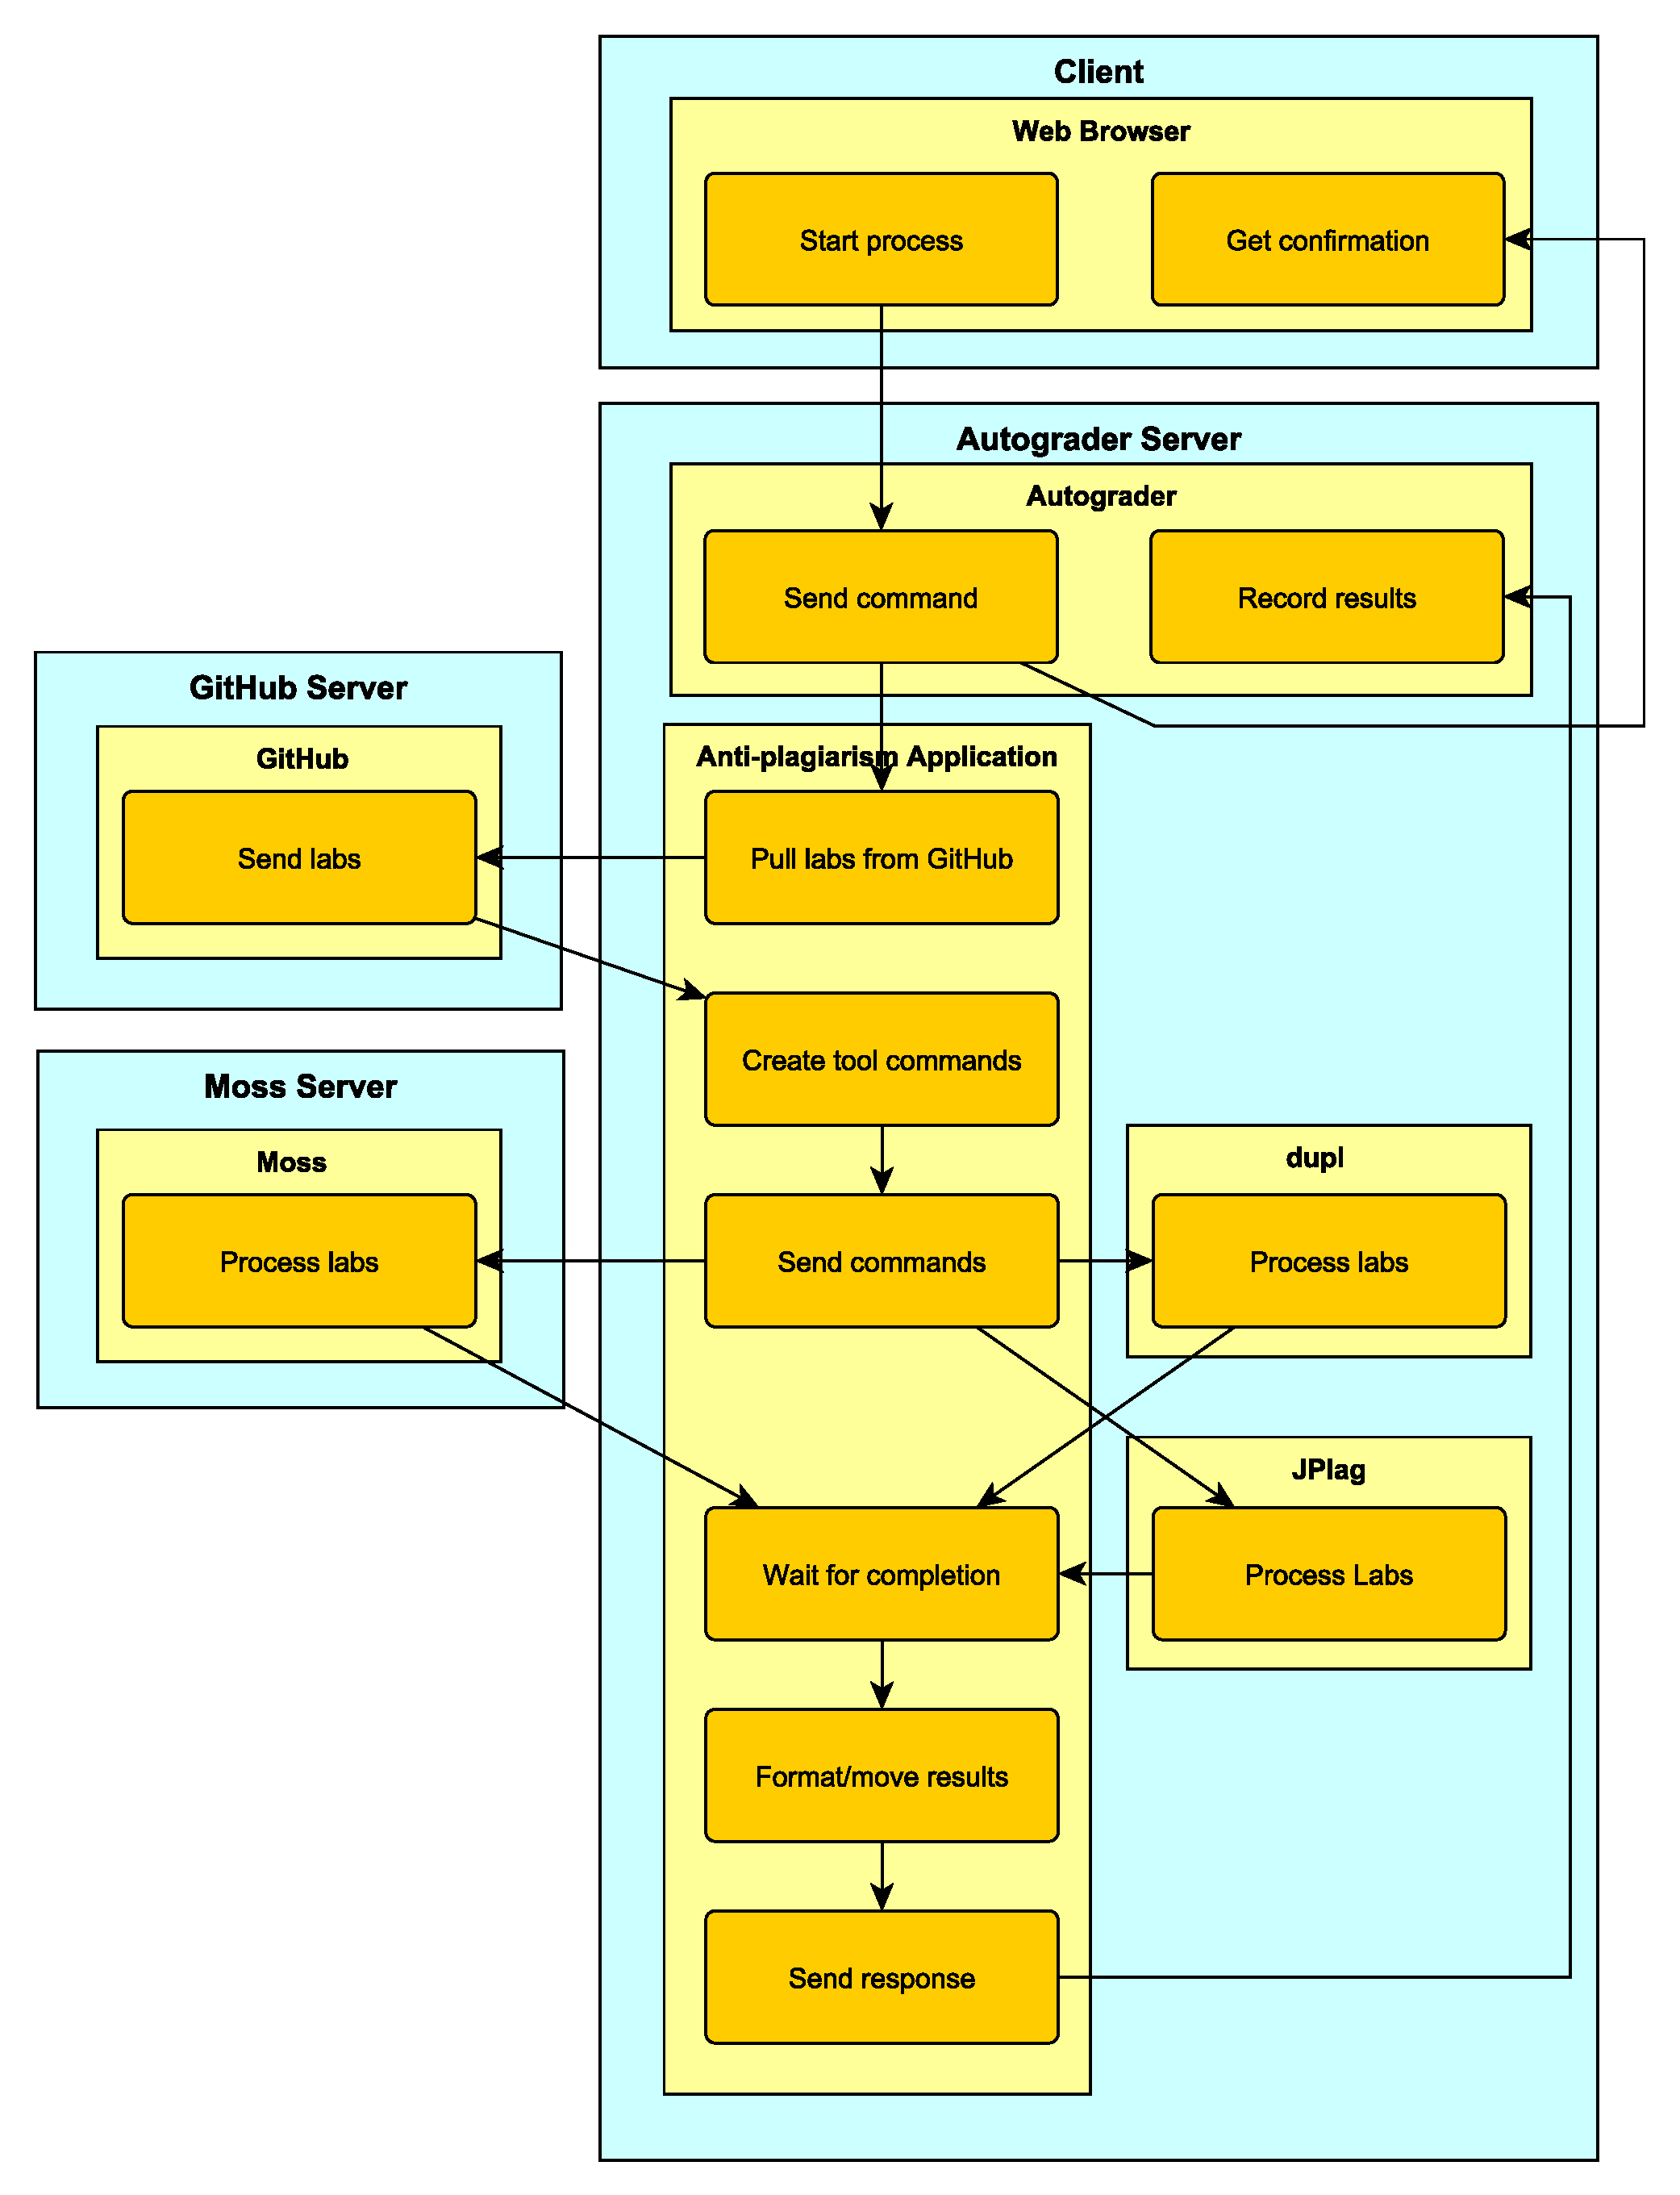
\includegraphics[width=1.0\textwidth]{process2.pdf}
			\caption{Process}
			\label{fig:process}
		\end{figure}
		
		Figure \ref{fig:process} shows how a request to the anti-plagiarism software is processed. When the Autograder web service receives a request to start the anti-plagiarism process, it creates the gRPC command. If it was successful it sends the request and informs the user that the request was sent. Since it can take at least several minutes to process the data, it is best to inform the user immediately that things might take a while. Otherwise they could think that it is not working. Then Autograder starts a Go routine (separate thread) to call the anti-plagiarism software and process the results. The gRPC call is synchronous, but it is not blocking Autograder from processing since it is in another thread.
	
		When the anti-plagiarism software receives the gRPC request, the students' code is pulled from GitHub to the Autograder server. Next the commands are created for each anti-plagiarism tools based on the location of the code, the language in which the code was written, the threshold of the tool, and various other parameters. The commands are then sent to their respective tools. Each student's work for an assignment is compared against the other students' work for that particular assignment in that class instead of all the assignments for that class or all the assignments for all classes. This keeps the number of files being compared from growing too large.
			
		The anti-plagiarism application waits for the results to come back from each of the tools. When they have all finished, the program will collect and store the resulting HTML files in the location specified. It also examines the HTML files for the highest incidents of plagiarism for each student. The highest values are written to a JSON file, which will be processed by Autograder. Finally the program sends a gRPC response back to the calling application indicating if it was successful or not.
		
	\section{Results}
	This sections presents the results of testing the anti-plagiarism software on real students' projects. It also describes the modification of parameters to improve the results.
	
		\subsection{Choosing threshold values}
		Choosing threshold values took some consideration plus trial and error. Since the threshold value for Moss is the number of files duplicate code can appear in and still be considered plagiarism, it was straightforward to find a value for Moss. The test class consisted of seventeen students and six groups. Therefore the Moss threshold would need to be less than six, because all of the groups would have code provided by the instructor. So the value chosen was five.
		
		For JPlag and dupl, the threshold represents the number of tokens to compare. It was not known how much data a token represents in JPlag, but luckily the output included the number of tokens in each match. In figure \ref{fig:jplag20} it is shown that 20 tokens can match short functions that only print a value. In figure \ref{fig:jplag30} it is shown that 30 tokens can match a long list of variable assignments. Figure \ref{fig:jplag40} shows that 40 tokens will match pieces of code that are more substantial. Therefore a JPlag threshold of 35 was chosen to get better matches.
		
		\begin{figure}[h!]
			\includegraphics[width=1.0\textwidth]{jplag20.png}
			\caption{JPlag match with 20 tokens.}
			\label{fig:jplag20}
		\end{figure}
		
		\begin{figure}[h!]
			\includegraphics[width=1.0\textwidth]{jplag30.png}
			\caption{JPlag match with 30 tokens.}
			\label{fig:jplag30}
		\end{figure}
		
		\begin{figure}[h!]
			\includegraphics[width=1.0\textwidth]{jplag40.png}
			\caption{JPlag match with 40 tokens.}
			\label{fig:jplag40}
		\end{figure}
		
		Unfortunately dupl does not provide the number of tokens in a match. So the threshold value needed to be adjusted several times before some of the less detailed results were removed. Figure \ref{fig:dupl50} and figure \ref{fig:dupl75} show examples of matches when the threshold was set to 50 and 75 respectively (up from the default value of 15). 75 was chosen for the final dupl threshold.
		
		\begin{figure}[h!]
			\includegraphics[width=1.0\textwidth]{dupl50.png}
			\caption{dupl match when threshold was 50 tokens.}
			\label{fig:dupl50}
		\end{figure}
		
		\begin{figure}[h!]
			\includegraphics[width=1.0\textwidth]{dupl75.png}
			\caption{dupl match when threshold was 75 tokens.}
			\label{fig:dupl75}
		\end{figure}
		
		\subsection{Results in Autograder}
		
		Figures \ref{fig:indlabresults} and \ref{fig:grouplabresults} show the individual lab results and group lab results respectively for the test class. In labs one, five, and six, the students programmed in C. They programmed in Go for the remaining labs. All of the test code for the labs was written in Go.  Light pink indicates that one tool found duplicate pieces of code, and darker pink indicates two tools found duplicates. Three tools finding results will not occur because there is no overlap in the languages that JPlag and dupl can test. Please note that the percentages shown here indicate the percentage of the assignment that the student has passed and not an amount of plagiarism.
		
		\begin{figure}[h!]
			\includegraphics[width=0.65\textwidth]{indlabresults.png}
			\caption{Individual lab results. Instructors and TAs have accounts too.}
			\label{fig:indlabresults}
		\end{figure}
		
		\begin{figure}[h!]
			\includegraphics[width=0.5\textwidth]{grouplabresults.png}
			\caption{Group lab results.}
			\label{fig:grouplabresults}
		\end{figure}
		
		An attempt was made to improve the results by manually deleting whole files that were common among the students. Partial files common among the students were not altered due to time constraints. The new results are listed in tables \ref{tab:newResults} and \ref{tab:newResults2}.
		
		\begin{table}[h!]
			\begin{center}
				\caption{Individual results after manually removing common whole files. M=Moss, J=JPlag, D=dupl}
				\label{tab:newResults}
				\begin{tabular}{ccccccccccccccc}
					\toprule
					Student & Lab 1 & Lab 2 & Lab 3 & Lab 4 & Lab 5\\
					\midrule
					1 & M & D & MD & D & \\
					2 &  &  & D & D & \\
					3 & M &  & D & D & \\
					4 &  &  & D & D & \\
					5 &  &  & MD & D & \\
					6 &  &  &  &  & \\
					7 &  &  & MD & D & \\
					8 & M &  & D & D & \\
					9 & M &  & D & D & \\
					10 &  & D & MD & MD & \\
					11 &  &  &  &  & \\
					12 & M &  & D &  & \\
					13 & M & D & D & D & \\
					14 &  & D & D & D & \\
					15 & M &  & D &  & \\
					16 & M &  & D & D & \\
					17 &  &  & MD & D & \\
					18 &  &  & MD & D & M\\
					19 &  &  & D & D & \\
					20 & M & D & D & D & \\
					21 &  & D & MD & D & \\
					22 &  &  & D & D & \\
					\bottomrule
				\end{tabular}
			\end{center}
		\end{table}
		
		\begin{table}[h!]
			\begin{center}
				\caption{Group results after manually removing common whole files. M=Moss, J=JPlag, D=dupl}
				\label{tab:newResults2}
				\begin{tabular}{ccccccccccccccc}
					\toprule
					Group & Lab 6 & Lab 7\\
					\midrule
					1 & MJ & MD\\
					2 &  & D\\
					3 & MJ & MD\\
					4 & MJ & MD\\
					5 & MJ & MD\\
					6 & J & D\\
					\bottomrule
				\end{tabular}
			\end{center}
		\end{table}
	
	\section{Analysis}
	This section analyzes the results of running the anti-plagiarism software against the real projects from Section 4. At first glance, it appeared as if all the students that submitted work plagiarized code, but that would be a very unlikely scenario. Most of the duplicates appear to come from code provided to the students. In labs one and five, little or no code was provided to the students. Therefore there were much fewer detections in these two assignments.
	
	Getting three separate tools to behave similarly using a common interface was a bit difficult. Moss was the original anti-plagiarism tool included in the project before it was decided to add other tools. Moss's threshold says to ignore code that is similar in a certain number of files. So if the threshold is ten and a piece of code appears at least ten times, it is not considered plagiarism. This is very helpful when an instructor gives students a partially completed file or a framework to follow. Since the threshold does not specify the length of code to consider for plagiarism, sometimes relatively short sections of code show up in the results. Unfortunately if a student's lab directory has subdirectories, Moss will say that similar code in different subdirectories is plagiarism.
	
	JPlag produces false positives because it does not currently ignore code provided by the instructor. It is possible to tell JPlag to ignore certain files. This is discussed further in Section 6.
	
	Dupl was not designed to detect plagiarism, only duplicate pieces of code. So it will detect all the instructor provided code as plagiarism. It can even detect two pieces of code in the same file. For example the two functions in figure \ref{fig:duplSameFile} are from the same file and are shown to be duplicates. Increasing the threshold helps with scenario though.
	
	\begin{figure}[h!]
		\includegraphics[width=0.5\textwidth]{duplSameFile2.png}
		\caption{Sample dupl results from same file.}
		\label{fig:duplSameFile}
	\end{figure}
	
	Since dupl is only looking for duplicate code and not plagiarism, it does not provide a number indicating the percentage of code it thinks is plagiarized. It also places all the results in a single HTML file rather than splitting them up into separate files.
	
	Adjustments were made to the thresholds in attempt to clean up the results shown in figures \ref{fig:indlabresults} and \ref{fig:grouplabresults}. Labs one and five improved some, but there was too much provided code in the other labs for cleaner results.
	
	By deleting common whole files shared by all the students, the results improved even more as seen in tables \ref{tab:newResults} and \ref{tab:newResults2}. The results could be improved further by handling the partial files shared by the students. All the labs except lab five had partially completed files. The partial files in labs one and two just had bare skeleton code, while the others had completed functions. Since the skeleton code is much smaller than the completed functions, it has less detections.
	
	\section{Future work}
	This section lists possible improvements to the anti-plagiarism software. Currently the application is only intended to be called locally, so there is no encryption enabled in the gRPC calls. If it is to be called remotely, then transport security needs to be added in the anti-plagiarism application and in Autograder. If the application was called remotely, the result files would need to be sent to the other machine. There are also some hard-coded values in Autograder that should be environment variables or in a configuration file, such as the address and port of the anti-plagiarism application.
	
	To improve the results from JPlag, a list of common files to ignore can be added. This will require changes to the Autograder GUI so that instructors can add the list to ignore. Also the gRPC request will need to be changed to include the list of files.
	
	The partial common files should also be handled in some way. Having the anti-plagiarism application remove the common pieces of code could be problematic because some tools require the code to be able to compile. Moss has the option to include base files. This could improve results from Moss, but Moss already seems to handle the situation well on its own. JPlag has an option for a base code directory, which may be worth looking into.
	
	\section{Conclusion}
	Due to the high number of false positives found during testing, it is probably better to consider the results from this application as supplemental to any suspicions an instructor may have already. It would be tedious to examine all of the results. The tools used are very good at finding similar pieces of code, but there are legitimate reasons for having duplicate code, such as code distributed by the instructor or students reusing their own code. Use of this application is useful if an instructor suspects plagiarism and uses this to verify their suspicions.
	
	Moss currently appears to be the best choice out of the three tools used in this project. Its ability to automatically ignore common code makes it easy to use. All of the tools were capable of finding duplicate pieces of code.
	
	Results could be improved in a several ways, such as adding a list of common files to ignore. With improved results, it would be much easier for instructors to look through the detections and find evidence of plagiarism.
	
	% use section* for acknowledgment
	\ifCLASSOPTIONcompsoc
		% The Computer Society usually uses the plural form
		\section*{Acknowledgments}
	\else
		% regular IEEE prefers the singular form
		\section*{Acknowledgment}
	\fi
	
	The author would like to thank Hein Meling for his advice and guidance during this project.
	
	\bibliography{sources}
	\bibliographystyle{ieeetr}

\begin{IEEEbiographynophoto}{Eric Scott Freeman}
is currently a master's student at the University of Stavanger. He received his Bachelor of Science degree in Computer Science from Midwestern State University in 2004. He has also worked as a software developer for several companies including RadioShack, Cisco Systems, and TelStrat.
\end{IEEEbiographynophoto}

\end{document}


